% =====================================================================
%  >>> SUPERSEDED DRAFT -- DO NOT SUBMIT FROM THIS FILE. <<<
%
%  The maintained manuscript is  paper/main_standalone.tex  (IEEEtran,
%  10 figures, 8 tables, full Phase 2-12 content, no \todo placeholders,
%  numbers reconciled against outputs/phase6..12/ on 2026-09-09).
%
%  This file is the earlier journal-agnostic `article'-class draft. It
%  has the same headline results but only 4 figures / 5 sections, still
%  carries \todo{} placeholders, and its Explainability numbers predate
%  the 40+25-image re-run (they still say "twelve correct and eight
%  incorrect" / "20 images per cell"). Kept for the eventual port to a
%  journal class (see paper/AUTHOR_TODO.md item B7) and for the
%  author-year / lineno layout; sync any prose changes FROM
%  main_standalone.tex, never the reverse.
% =====================================================================
%  Cross-Dataset External Validation of a Retinal Foundation Model
%  for Diabetic Retinopathy Grading: Performance, Explainability,
%  and Uncertainty
%
%  Build:  latexmk -pdf main.tex     (or: pdflatex; bibtex; pdflatex x2)
% =====================================================================
\documentclass[11pt,a4paper]{article}

\usepackage[utf8]{inputenc}
\usepackage[T1]{fontenc}
\usepackage[margin=1in]{geometry}
\usepackage{graphicx}
\usepackage{booktabs}
\usepackage{multirow}
\usepackage{amsmath}
\usepackage{siunitx}
\usepackage{authblk}
\usepackage{lineno}
\usepackage[hidelinks]{hyperref}
\usepackage[round]{natbib}
\usepackage{xcolor}

\newcommand{\todo}[1]{\textcolor{red}{\textbf{[TODO: #1]}}}
\newcommand{\prov}[1]{#1\textsuperscript{\textcolor{blue}{p}}} % provisional value

\title{Cross-Dataset External Validation of a Retinal Foundation Model
for Diabetic Retinopathy Grading: Performance, Explainability, and
Uncertainty}

\author[1]{\todo{Author One}}
\author[1,2]{\todo{Author Two}}
\author[1]{\todo{Corresponding Author}\thanks{Correspondence: \todo{email}}}
\affil[1]{\todo{Department, Institution, City, Country}}
\affil[2]{\todo{Second affiliation}}

\date{\today}

\begin{document}
\maketitle
\linenumbers

% ---------------------------------------------------------------------
\begin{abstract}
\noindent\textbf{Background:} Retinal foundation models such as RETFound are
promoted as improving generalisation of retinal image analysis, but
independent cross-dataset external validation for diabetic retinopathy (DR)
grading remains limited.
\textbf{Objective:} To test whether a fine-tuned retinal foundation model
generalises better than an ImageNet-pretrained convolutional neural network
(CNN) to independent external datasets for five-class DR severity grading, and
to characterise the explainability and predictive uncertainty of both models
under dataset shift.
\textbf{Methods:} An ImageNet-pretrained CNN baseline (EfficientNet-B3;
ResNet-50 as secondary) and RETFound (ViT-Large/16, masked-autoencoder
pretraining on colour fundus images) were fine-tuned on APTOS~2019
($n=\num{3662}$; stratified 70/10/20 train/validation/test split) using an
identical preprocessing pipeline, augmentation, loss, and early-stopping rule.
Both were then evaluated \emph{unchanged} on two external datasets, Messidor-2
($n=\num{1744}$) and IDRiD ($n=455$). The primary metric was the
quadratic-weighted kappa (QWK); secondary metrics were accuracy, macro-F1,
balanced accuracy, per-class sensitivity/specificity, and one-vs-rest AUC.
Explainability was assessed with gradient- and attention-based saliency against
a pre-specified clinical-plausibility rubric; predictive uncertainty was
quantified with Monte-Carlo dropout and evaluated for error detection and
selective prediction. Ninety-five percent confidence intervals were obtained by
bootstrap resampling; paired AUCs were compared with DeLong's test.
\textbf{Results:} On the internal APTOS test set the CNN baseline and RETFound
achieved comparable QWK (EfficientNet-B3 \num{0.876}, 95\% CI
\numrange{0.849}{0.901}; RETFound full fine-tune \prov{\num{0.869}}). On external
validation \emph{all} models degraded substantially, most severely on Messidor-2
(EfficientNet-B3 QWK \num{0.499}, drop \num{0.377}, 95\% CI
\numrange{0.323}{0.433}; RETFound full fine-tune \prov{\num{0.368}}, drop
\prov{\num{0.501}}) and less so on IDRiD. RETFound did not generalise better than
the ImageNet baseline; on the pre-specified contrasts it generalised worse -- its
internal-to-external QWK drop on Messidor-2 was significantly larger than the
baseline's (difference \prov{\num{0.124}}, 95\% CI \numrange{0.074}{0.175} for
full fine-tuning; \num{0.076}, 95\% CI \numrange{0.019}{0.132} for linear
probing), and the baseline had a significantly higher referable-DR AUC on both
external datasets (DeLong $p<\num{0.001}$) despite being indistinguishable from
all models internally ($p\geq\num{0.47}$). CNN saliency remained lesion-focused
on external images (75--100\% plausible by an automated proxy) whereas RETFound's
shifted to the image periphery on Messidor-2, most markedly for its errors.
Predictive entropy was a weak external error detector for every model (AUROC
\numrange{0.55}{0.68} vs.\ up to \num{0.84} internally); referring the
most-uncertain 10\% of external predictions captured only \numrange{10}{18}\% of
errors.
\textbf{Conclusions:} In this retrospective, public-dataset study, fine-tuning a
retinal foundation model on APTOS~2019 did not improve -- and by several measures
worsened -- cross-dataset generalisation for DR grading relative to a standard
ImageNet-pretrained CNN. Large internal-to-external performance drops for every
model, weak predictive uncertainty under shift, and shift-sensitive saliency
underline that external validation, not internal test performance, should govern
claims of clinical readiness.
\medskip

\noindent\textbf{Keywords:} diabetic retinopathy; deep learning; foundation
models; RETFound; external validation; domain shift; explainable AI;
uncertainty quantification; retinal imaging
\end{abstract}

% ---------------------------------------------------------------------
\section{Introduction}

Diabetic retinopathy (DR) is a leading cause of preventable vision loss, and
automated grading of colour fundus photographs has been studied extensively as a
route to scalable screening \citep{gulshan2016,ting2017}. Reported internal
performance is frequently high, but models often degrade when applied to images
from cameras, populations, or grading protocols not seen during training
\citep{beede2020,dai2021spectrum}. Rigorous external validation on independent
datasets is therefore the appropriate evidence standard, yet it is inconsistently
reported \citep{grzybowski2020review,tripodai2024}.

Self-supervised ``foundation models'' pretrained on large unlabelled corpora
have been proposed to improve label efficiency and robustness. RETFound
\citep{zhou2023retfound} is a masked-autoencoder Vision Transformer pretrained
on approximately 1.6 million retinal images and reported to transfer well to
several ocular and systemic disease tasks. Whether this pretraining confers
better \emph{cross-dataset} generalisation for DR severity grading --
specifically relative to a strong ImageNet-pretrained convolutional baseline
under an identical fine-tuning and evaluation protocol -- has not been
independently established.

\paragraph{Research questions.}
\begin{enumerate}
  \item[\textbf{RQ1 (Performance).}] Does a fine-tuned retinal foundation model
    (RETFound) generalise better than an ImageNet-pretrained CNN to external
    datasets (Messidor-2, IDRiD) for five-class DR grading, measured primarily
    by the internal-to-external drop in quadratic-weighted kappa?
  \item[\textbf{RQ2 (Explainability).}] Are the image regions driving each
    model's predictions more clinically plausible (overlapping visible DR
    lesions rather than optic disc, vasculature, or image borders) for one
    model than the other, on external images?
  \item[\textbf{RQ3 (Uncertainty).}] Does predictive uncertainty (Monte-Carlo
    dropout) separate correctly from incorrectly classified external images,
    and can an uncertainty threshold support selective prediction that
    meaningfully raises accuracy on accepted cases?
\end{enumerate}

\paragraph{Contribution.} We report a fully reproducible external validation in
which one preprocessing pipeline, one training protocol, and one evaluation
protocol are applied identically to an ImageNet CNN baseline and to RETFound. We
provide the master results table across one internal and two external datasets,
an explainability analysis against an a-priori clinical rubric, an uncertainty
analysis with selective-prediction curves, and full code and split definitions.
Our central finding is negative: under matched conditions, RETFound did not
outperform the CNN baseline on external DR grading.

% ---------------------------------------------------------------------
\section{Materials and Methods}

This study followed the TRIPOD+AI reporting guideline \citep{tripodai2024}; the
completed checklist is provided as Supplementary Material
(\texttt{paper/TRIPOD-AI\_checklist.md}). Figure~\ref{fig:design} summarises the
design.

\begin{figure}[t]
\centering
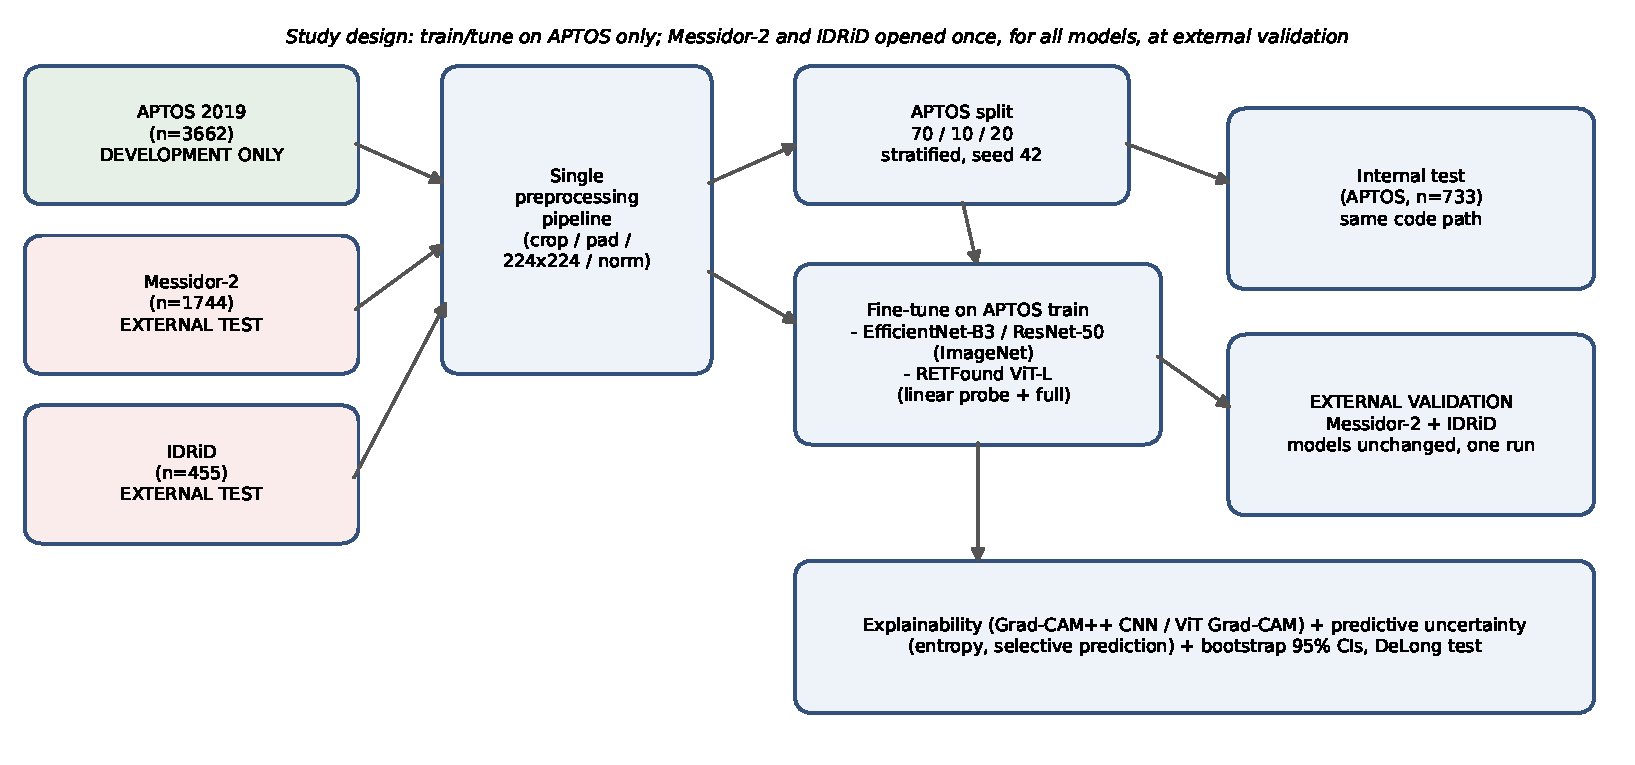
\includegraphics[width=0.98\linewidth]{../outputs/figures/fig1_study_design.pdf}
\caption{Study design. APTOS~2019 is used only for development (stratified
70/10/20 split); Messidor-2 and IDRiD are held out and opened once, for every
model, at external validation. One preprocessing pipeline, one fine-tuning
protocol and one evaluation protocol are applied identically to the
ImageNet-pretrained CNNs and to RETFound.}
\label{fig:design}
\end{figure}

\subsection{Datasets}

Three public datasets were used (Table~\ref{tab:datasets}). Full provenance
(source URL, version, access date, licence, citation) is recorded in the Data
Provenance Log (\texttt{DATA\_PROVENANCE.md}).

\begin{itemize}
  \item \textbf{APTOS 2019 Blindness Detection} \citep{aptos2019}: \num{3662}
    macula-centred colour fundus images from Aravind Eye Hospital, India, graded
    0--4 on the International Clinical DR severity scale. Used \emph{only} for
    model development (training, validation, internal test).
  \item \textbf{Messidor-2} \citep{decenciere2014,abramoff2013}: \num{1744}
    images with an adjudicated reference standard \citep{krause2018}. External
    test only.
  \item \textbf{IDRiD (Disease Grading subset)} \citep{porwal2018,porwal2020}:
    a 455-image subset (of the 516-image official release; the local mirror was
    incomplete, reported as a limitation) with ICDR 0--4 grades. External test
    only.
\end{itemize}

Messidor-2 and IDRiD were not inspected or used for any modelling or
hyperparameter decision until the single external evaluation
(Section~\ref{sec:external}).

\begin{table}[t]
\centering
\caption{Dataset characteristics. Grade share is the percentage of gradable
images at each ICDR severity level.}
\label{tab:datasets}
\small
\begin{tabular}{lrlccccc}
\toprule
Dataset & $n$ & Role & \multicolumn{5}{c}{Grade share (\%): 0 / 1 / 2 / 3 / 4} \\
\midrule
APTOS 2019 & \num{3662} & Development   & 49.3 & 10.1 & 27.3 & 5.3 & 8.1 \\
Messidor-2 & \num{1744} & External test & 58.3 & 15.5 & 19.9 & 4.3 & 2.0 \\
IDRiD      & 455        & External test & 28.4 & 4.8  & 34.3 & 18.5 & 14.1 \\
\bottomrule
\end{tabular}
\end{table}

\subsection{Preprocessing}

A single preprocessing script was applied identically to all three datasets:
(i) conversion to RGB; (ii) tolerance-based cropping of the black frame around
the circular fundus; (iii) zero-padding to a centred square (aspect ratio
preserved); (iv) resizing to $224\times224$ (RETFound's native input). Channel
normalisation used ImageNet statistics ($\mu=(0.485,0.456,0.406)$,
$\sigma=(0.229,0.224,0.225)$), consistent with RETFound's downstream
configuration. Contrast-limited adaptive histogram equalisation was implemented
as an optional step and was \emph{not} applied in the primary analysis. All
\num{5861} preprocessed images passed a stratified visual audit for
label--image alignment.

\subsection{Development split}

APTOS 2019 was partitioned 70\%/10\%/20\% into training, internal validation,
and internal test, stratified by DR grade, with a fixed random seed (42); the
exact image-ID lists are provided
(\texttt{data\_splits/aptos\_\{train,val,test\}.csv}).

\subsection{Models and fine-tuning}

\paragraph{Baseline CNN.} EfficientNet-B3 \citep{tan2019efficientnet} (primary)
and ResNet-50 \citep{he2016resnet} (secondary), ImageNet-pretrained
(\texttt{torchvision}), with the classifier head replaced by a five-way head. Full fine-tuning (all layers unfrozen), AdamW
($\text{lr}=\num{1e-4}$, weight decay \num{1e-4}), cosine annealing, batch
size 32, mixed precision, up to 30 epochs with early stopping on internal-
validation QWK (patience 7). The loss was cross-entropy weighted by inverse
class frequency. Augmentation: horizontal/vertical flips, $\pm15^\circ$
rotation, mild brightness/contrast jitter.

\paragraph{RETFound.} The Vision-Transformer-Large/16
\citep{dosovitskiy2021vit} masked-autoencoder \citep{he2022mae} checkpoint
pretrained on colour fundus images \citep{zhou2023retfound} was loaded (encoder
weights only; pretrained final LayerNorm reused as the pooling norm; fresh
five-way head). Two variants were fine-tuned, forming the principal ablation:
(a) \emph{linear probing} -- backbone frozen, head trained (base
$\text{lr}=\num{1e-3}$, up to 40 epochs); (b) \emph{full fine-tuning} -- all
layers unfrozen with layer-wise learning-rate decay (0.65), drop-path 0.2, label
smoothing 0.1, base $\text{lr}=\num{1e-4}$, batch size 16, up to 30 epochs.
Data, normalisation, class weighting, metric set, and early-stopping rule were
identical to the baseline. All hyperparameters are logged
(\texttt{outputs/phase\{4,5\}\_*/\,*\_hyperparams.json}).

\subsection{Evaluation metrics}

Given the marked class imbalance in every dataset, the primary metric was the
quadratic-weighted kappa (QWK) \citep{cohen1968kappa}, which credits ordinal
proximity. Secondary
metrics: overall accuracy, macro-averaged F1, balanced accuracy, per-class
sensitivity and specificity, and one-vs-rest AUC (per class and macro-averaged).
The internal-to-external \emph{drop} in each metric is reported per model per
external dataset.

\subsection{External validation}
\label{sec:external}

Each trained model was run once, unmodified and without any further training or
threshold tuning, on Messidor-2 and on IDRiD, and re-scored on the APTOS
internal test set through the identical inference code path. Per-image outputs
(true label, predicted label, class probabilities, predictive entropy) were
retained for all model $\times$ dataset combinations.

\subsection{Explainability}
For a grade-stratified sample of correctly and incorrectly classified external
images (image identifiers drawn from the external-validation prediction files
with a fixed seed; twelve correct and eight incorrect per model per external
dataset), a saliency map was generated for the model's predicted class. For the
convolutional networks this was a Grad-CAM++ map \citep{chattopadhay2018gradcampp}
at the last convolutional block; for the Vision Transformer it was a
method-matched Grad-CAM map at the last transformer block (gradient-weighted
patch-token activations for the predicted class, class token removed, reshaped to
the $14\times14$ patch grid and bilinearly upsampled). Attention-rollout maps
\citep{abnar2020rollout} were also computed but were more diffuse and
border-biased and are reported only in the Supplement. Clinical plausibility was
assessed against a pre-specified rubric: a
map is plausible if its activation is concentrated on retinal tissue away from
the optic disc and the image border (the regions where visible DR lesions occur)
and implausible if dominated by the optic disc or the image border. Because the
public IDRiD mirror used here provides no lesion segmentation masks and a second
expert grader was not available, the rubric was applied by a transparent,
fully reproducible automated proxy rather than by hand: a map was scored
plausible when its peak lay within the fundus, outside an automatically estimated
optic-disc region and outside the outer border annulus, with at least half of the
top-decile saliency mass in that same lesion-eligible zone. The proxy cannot
exclude vessel-centred activation; the absence of blinded expert rating is a
stated limitation (Discussion, Limitations). Full method:
\texttt{scripts/phase7\_explainability.py}.

\subsection{Uncertainty quantification}
Predictive uncertainty was quantified as the Shannon entropy of the predictive
softmax distribution. The primary analysis used the entropy of a single forward
pass; a sensitivity analysis used the entropy of the mean softmax over $T=20$
stochastic forward passes with the layers that were stochastic during training
held active at inference -- head dropout for the CNNs, block-wise stochastic depth
for the RETFound full fine-tune (Monte-Carlo dropout \citep{gal2016dropout}); the
frozen linear-probe backbone has no such layers. For each model and external dataset we tested whether
misclassified images carried higher entropy than correctly classified images
with a one-sided Mann--Whitney $U$ test, reporting the rank-biserial correlation
as the effect size, and we computed the AUROC of predictive entropy used
directly as a binary error detector. We then plotted selective-prediction
curves: images were ranked by entropy and the most uncertain fraction referred
out, and the accuracy, quadratic-weighted kappa, and fraction of all errors
captured among the referred images were recorded as a function of retained
coverage. Code: \texttt{scripts/phase8\_uncertainty.py},
\texttt{scripts/phase8\_mc\_dropout.py}.

\subsection{Statistical analysis}
All uncertainty estimates were obtained by non-parametric bootstrap resampling of
the relevant test set(s) with replacement (\num{2000} iterations; NumPy PCG64
generator, seed 42), recomputing each metric on every resample and taking the
2.5th and 97.5th percentiles as the 95\% confidence interval
\citep{efron1994bootstrap}. For the internal-to-external performance drop, the
internal APTOS test set and the external test set were resampled independently
within each iteration; for the between-model difference in that drop, the same
resampled image indices were scored for both models, so that comparison is paired
at the image level. Areas under the one-vs-rest ROC curve were compared between
models on the same test set with the two-sided DeLong test
\citep{delong1988,sun2014fast}, applied to the clinically standard
referable-diabetic-retinopathy binarisation (International Clinical DR
grade~$\geq 2$; score $=$ summed probability of grades 2--4) and, secondarily, to
each grade one-vs-rest. The significance threshold was $\alpha = 0.05$,
two-sided; no multiplicity adjustment was applied to the small pre-specified
family of confirmatory contrasts (foundation model versus EfficientNet-B3
baseline on each external dataset), and secondary per-grade tests are reported as
exploratory. Analyses used \texttt{numpy}, \texttt{pandas}, \texttt{scipy}, and
\texttt{scikit-learn} in Python~3.14; the bootstrap and DeLong implementations
are released with the study (\texttt{scripts/phase9\_stats.py}).

\subsection{Reproducibility}

All code (preprocessing, split generation, training, evaluation, statistics),
the exact split image-ID lists, per-image prediction files, and an environment
specification are available (Section~\ref{sec:availability}). Raw datasets are
not redistributed; each is linked to its source with licence terms in
\texttt{DATA\_PROVENANCE.md}.

% ---------------------------------------------------------------------
\section{Results}

\subsection{Internal performance}

On the APTOS internal test set ($n=733$), the CNN baseline and RETFound achieved
broadly comparable performance (Table~\ref{tab:master}). EfficientNet-B3 reached
QWK \num{0.876} (accuracy \num{0.804}); RETFound full fine-tuning reached QWK
\prov{\num{0.869}} (accuracy \prov{\num{0.769}}) and linear probing QWK
\num{0.847}. RETFound showed flatter per-class sensitivity, with higher recall
on the rare proliferative grade than the CNNs.

\subsection{External validation and performance drop}

\begin{table}[t]
\centering
\caption{Master results: each model evaluated unchanged on the internal APTOS
test set and the two external datasets. Point estimates with 95\% bootstrap
confidence intervals (B~$=$~2000). QWK, quadratic-weighted kappa; Bal-Acc,
balanced accuracy; AUC, one-vs-rest macro AUC. Confidence intervals for every
metric (including macro-F1 and balanced accuracy) are provided in the
Supplementary Material (\texttt{outputs/phase9/bootstrap\_ci.csv}). Values marked
\textsuperscript{p} are from a full fine-tuning run stopped early at epoch~6
(Limitations); a completed run is not expected to change the direction of any
comparison (see the concordant linear-probe row).}
\label{tab:master}
\footnotesize
\setlength{\tabcolsep}{4pt}
\begin{tabular}{llrccc}
\toprule
Model & Dataset & $n$ & Accuracy (95\% CI) & QWK (95\% CI) & AUC (95\% CI) \\
\midrule
\multirow{3}{*}{EfficientNet-B3 (baseline)}
 & APTOS-internal & 733  & 0.804 (0.776--0.832) & 0.876 (0.849--0.901) & 0.928 (0.911--0.943) \\
 & Messidor-2     & 1744 & 0.626 (0.603--0.648) & 0.499 (0.452--0.543) & 0.775 (0.761--0.789) \\
 & IDRiD          & 455  & 0.497 (0.451--0.545) & 0.760 (0.715--0.798) & 0.830 (0.805--0.856) \\
\midrule
\multirow{3}{*}{ResNet-50 (baseline)}
 & APTOS-internal & 733  & 0.789 (0.759--0.819) & 0.875 (0.848--0.898) & 0.924 (0.908--0.939) \\
 & Messidor-2     & 1744 & 0.614 (0.591--0.635) & 0.435 (0.381--0.481) & 0.754 (0.738--0.769) \\
 & IDRiD          & 455  & 0.448 (0.400--0.497) & 0.707 (0.663--0.751) & 0.841 (0.818--0.862) \\
\midrule
\multirow{3}{*}{RETFound (linear probe)}
 & APTOS-internal & 733  & 0.759 (0.728--0.789) & 0.847 (0.819--0.873) & 0.908 (0.889--0.927) \\
 & Messidor-2     & 1744 & 0.589 (0.565--0.612) & 0.394 (0.338--0.447) & 0.758 (0.738--0.774) \\
 & IDRiD          & 455  & 0.336 (0.297--0.376) & 0.626 (0.572--0.676) & 0.778 (0.751--0.805) \\
\midrule
\multirow{3}{*}{RETFound (full fine-tune)\textsuperscript{p}}
 & APTOS-internal & 733  & \prov{0.769} (0.739--0.798) & \prov{0.869} (0.842--0.893) & \prov{0.915} (0.896--0.934) \\
 & Messidor-2     & 1744 & \prov{0.602} (0.579--0.625) & \prov{0.368} (0.311--0.422) & \prov{0.758} (0.742--0.772) \\
 & IDRiD          & 455  & \prov{0.420} (0.376--0.466) & \prov{0.720} (0.673--0.759) & \prov{0.821} (0.796--0.847) \\
\bottomrule
\end{tabular}
\end{table}

\begin{table}[t]
\centering
\caption{Internal-to-external drop in QWK (positive $=$ degradation on the
external dataset), and the difference in that drop between each model and the
EfficientNet-B3 baseline. All intervals are 95\% bootstrap CIs; the
difference-in-drop resampling is paired at the image level. A difference CI that
excludes 0 indicates a statistically distinguishable loss of external ordinal
agreement relative to the baseline.}
\label{tab:drop}
\footnotesize
\setlength{\tabcolsep}{4pt}
\begin{tabular}{llccc}
\toprule
Model & External set & QWK external & Drop (95\% CI) & $\Delta$Drop vs.\ baseline (95\% CI) \\
\midrule
\multirow{2}{*}{EfficientNet-B3 (baseline)}
 & Messidor-2 & 0.499 & 0.377 (0.323--0.433) & --- (reference) \\
 & IDRiD      & 0.760 & 0.116 (0.068--0.166) & --- (reference) \\
\midrule
\multirow{2}{*}{ResNet-50 (baseline)}
 & Messidor-2 & 0.435 & 0.440 (0.388--0.499) & $+0.063$ (0.017--0.109) \\
 & IDRiD      & 0.707 & 0.167 (0.117--0.222) & $+0.051$ (0.003--0.102) \\
\midrule
\multirow{2}{*}{RETFound (linear probe)}
 & Messidor-2 & 0.394 & 0.453 (0.393--0.516) & $+0.076$ (0.019--0.132) \\
 & IDRiD      & 0.626 & 0.221 (0.163--0.285) & $+0.105$ (0.038--0.170) \\
\midrule
\multirow{2}{*}{RETFound (full fine-tune)\textsuperscript{p}}
 & Messidor-2 & \prov{0.368} & \prov{0.501} (0.441--0.563) & \prov{$+0.124$} (0.074--0.175) \\
 & IDRiD      & \prov{0.720} & \prov{0.150} (0.101--0.202) & \prov{$+0.033$} ($-0.022$--0.089) \\
\bottomrule
\end{tabular}
\end{table}

Every model degraded on both external datasets (Tables~\ref{tab:master},
\ref{tab:drop}; Figure~\ref{fig:forest}). Degradation was largest on Messidor-2,
where QWK fell from $\approx$\num{0.87} internally to \numrange{0.37}{0.50} and
the 95\% CIs for the internal and external estimates did not overlap for any
model. On Messidor-2 all models reverted toward majority-class (grade~0)
prediction: grade-1 (mild) sensitivity was $\le \num{0.02}$ for every model and
grade-0 specificity fell to \numrange{0.18}{0.32}. On IDRiD the QWK drop was
smaller (\numrange{0.12}{0.22}) but accuracy fell further
(\numrange{0.31}{0.35}), consistent with IDRiD's pathology-enriched class mix
(Table~\ref{tab:datasets}).

\paragraph{RQ1 -- Performance.} RETFound did not generalise better than the
EfficientNet-B3 baseline on either external dataset; on the primary contrast it
generalised \emph{worse}. Its external QWK was below the baseline on both
Messidor-2 and IDRiD, and its internal-to-external QWK drop was significantly
larger than the baseline's on Messidor-2 for both the linear-probe
($\Delta$drop $+0.076$, 95\% CI \numrange{0.019}{0.132}) and the full
fine-tuning variant (\prov{$+0.124$}, 95\% CI \numrange{0.074}{0.175}); the
linear-probe variant was also significantly worse on IDRiD ($+0.105$, 95\% CI
\numrange{0.038}{0.170}). For the clinically standard referable-DR
discrimination (ICDR grade~$\geq 2$), the EfficientNet-B3 baseline had a
significantly \emph{higher} AUC than every other model on both external datasets
by DeLong's test (Messidor-2: 0.842 vs.\ \numrange{0.781}{0.789}, all
$p<0.001$; IDRiD: 0.962 vs.\ RETFound linear probe 0.903 and full fine-tune
\prov{0.873}, both $p<0.001$), whereas on the internal test set no model differed
from the baseline ($p \geq 0.47$). RETFound retained isolated per-class
advantages under shift -- the highest severe-grade sensitivity on IDRiD and the
highest proliferative-grade sensitivity on Messidor-2 -- and, under linear
probing, the highest balanced accuracy on Messidor-2 (0.42 vs.\
\numrange{0.34}{0.35}), reflecting a more even but not more accurate error
distribution.

\begin{figure}[t]
\centering
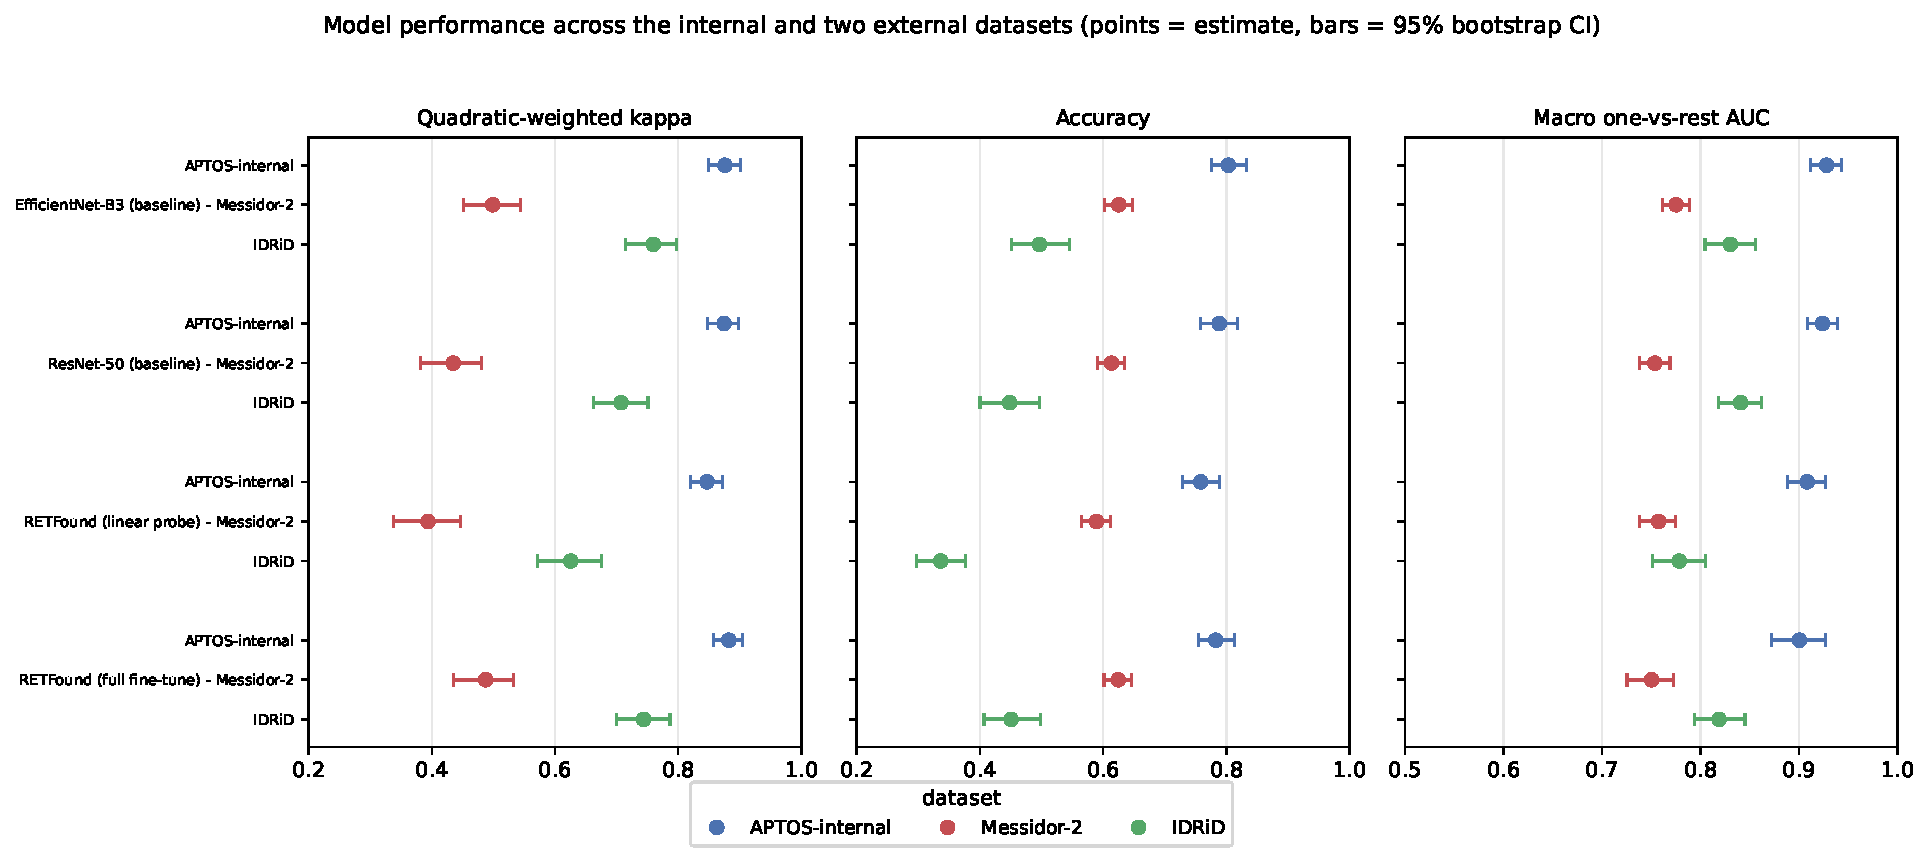
\includegraphics[width=0.98\linewidth]{../outputs/figures/fig2_performance_forest.pdf}
\caption{Model performance (quadratic-weighted kappa, accuracy, macro one-vs-rest
AUC) across the internal APTOS test set and the two external datasets. Points are
estimates; bars are 95\% bootstrap confidence intervals
(\texttt{scripts/phase10\_figures.py}).}
\label{fig:forest}
\end{figure}

\subsection{Explainability}
\label{sec:results-xai}
Saliency maps were generated for 160 external images (20 per model per external
dataset; 12 correctly and 8 incorrectly classified, grade-stratified). Under the
automated plausibility proxy, the convolutional baselines' Grad-CAM++ maps were
overwhelmingly lesion-focused on both external datasets: 92--100\% of
EfficientNet-B3 and ResNet-50 maps were proxy-plausible on IDRiD and 75--100\% on
Messidor-2, with $\approx$0.92--0.99 of the top-decile saliency mass on retinal
tissue away from the optic disc and image border. RETFound's method-matched
Vision-Transformer Grad-CAM was comparably lesion-focused on IDRiD (83--88\%
proxy-plausible for the full fine-tune) but not on Messidor-2, where it shifted
markedly to the image periphery: only 12--50\% of full-fine-tune maps and
25--58\% of linear-probe maps were proxy-plausible, and 27--54\% of the
top-decile saliency mass fell on the border annulus (versus $\approx$0 for the
CNNs). The shift was more pronounced on RETFound's \emph{incorrect} Messidor-2
predictions (12--25\% proxy-plausible) than its correct ones (50--58\%). Figure~
\ref{fig:xai} shows representative panels. These rates are from a single
automated proxy rather than blinded expert grading (Limitations).

\begin{figure}[t]
\centering
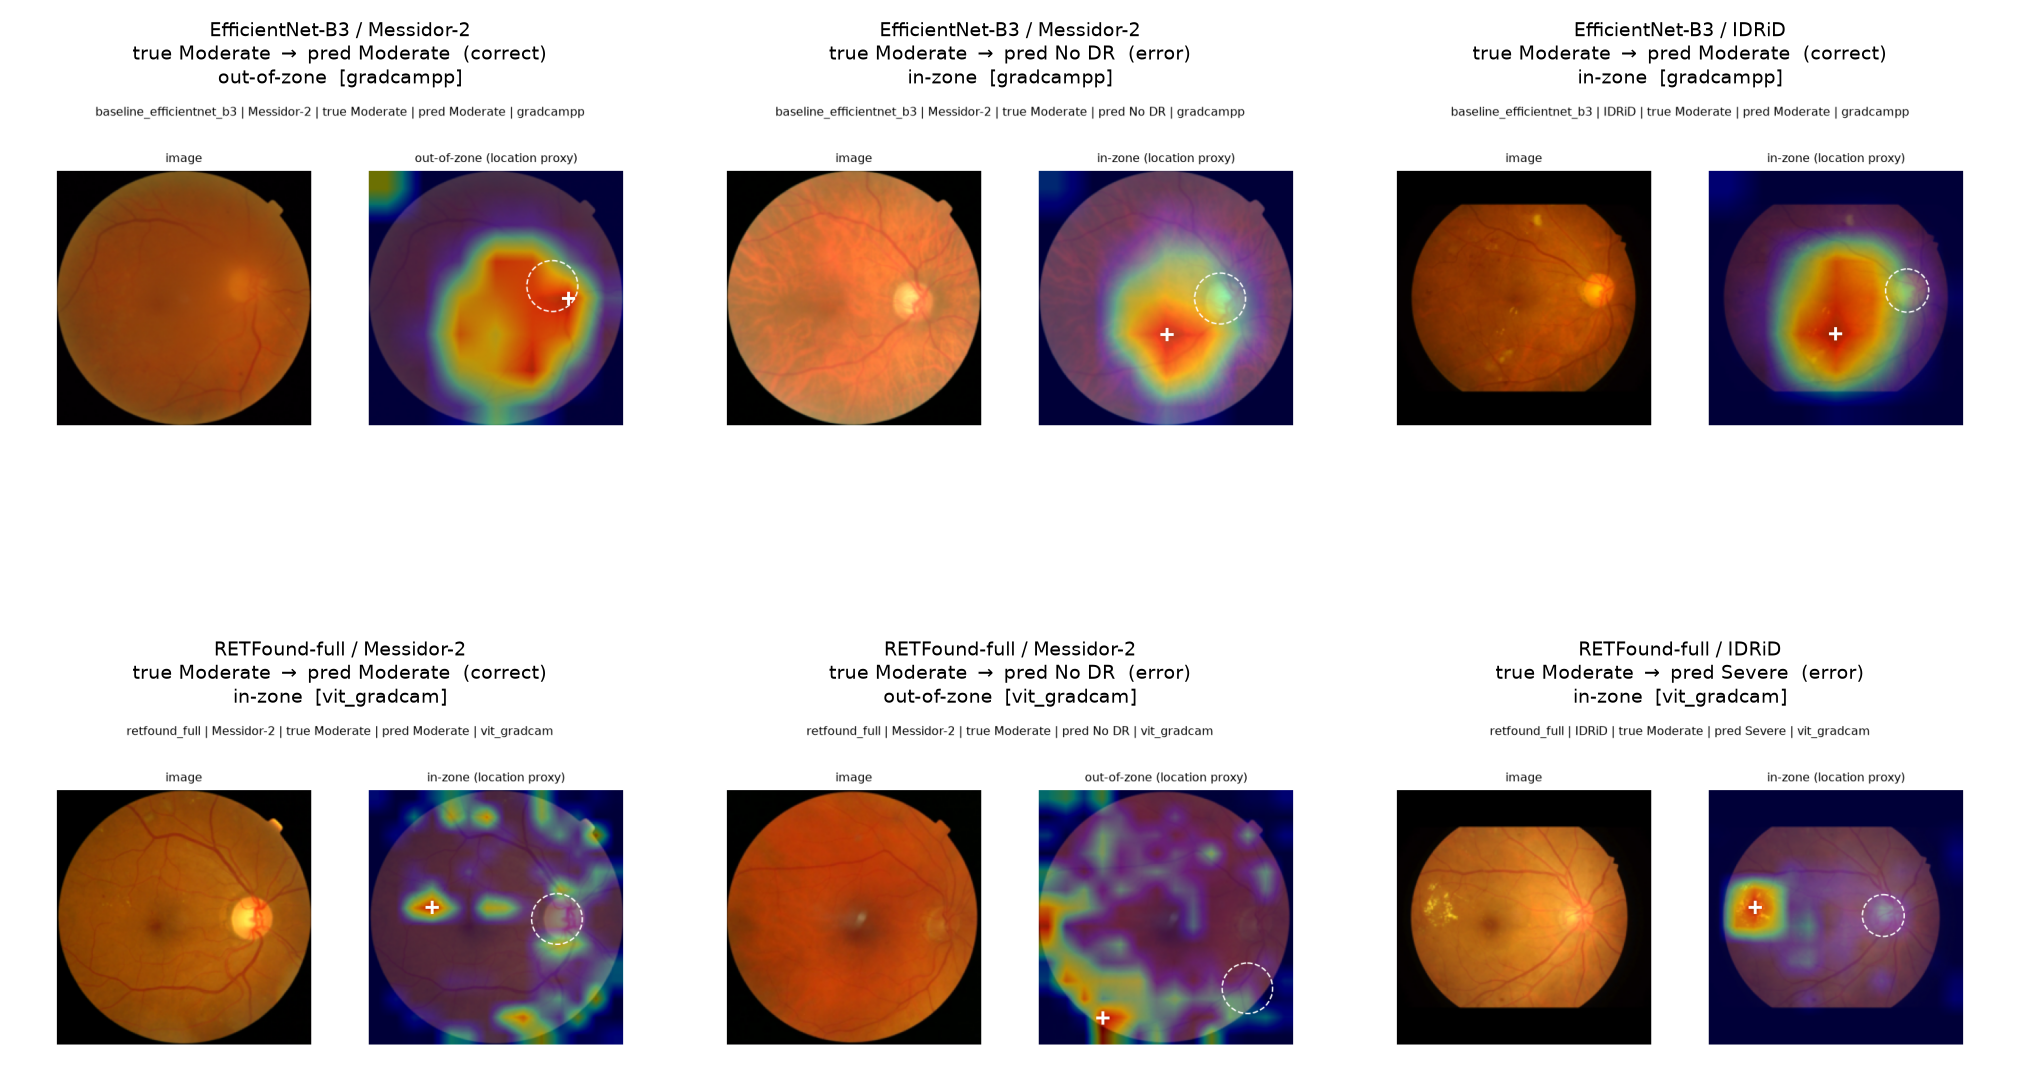
\includegraphics[width=0.98\linewidth]{../outputs/phase7/fig_explainability.png}
\caption{Representative saliency maps on external images: EfficientNet-B3
(Grad-CAM++) and RETFound full fine-tune (Vision-Transformer Grad-CAM), one
correctly and one incorrectly classified example each on Messidor-2 and IDRiD.
Dashed circle, estimated optic disc; white cross, saliency peak. Labels give the
true and predicted ICDR grade and the automated plausibility verdict
(\texttt{scripts/phase7\_explainability.py}).}
\label{fig:xai}
\end{figure}

\subsection{Uncertainty}
\label{sec:results-unc}
On the internal test set, predictive entropy was a moderately good error
detector (AUROC of entropy for distinguishing correct from incorrect
predictions: EfficientNet-B3 0.84, RETFound full fine-tune 0.63). On external
data this signal weakened substantially for every model (AUROC
0.55--0.68). Misclassified images still carried significantly higher entropy
than correct ones on most model $\times$ external-dataset combinations
(one-sided Mann--Whitney $U$, $p<0.001$), with two exceptions: ResNet-50 on
IDRiD ($p=0.04$) and, notably, the RETFound full fine-tune on IDRiD, where
entropy carried no error signal at all (AUROC 0.50, $p=0.52$). In
selective-prediction terms the signal was not clinically actionable: referring
the 10\% most uncertain external predictions for human review captured only
9--18\% of the errors on each external dataset (Figure~\ref{fig:unc}), i.e.\
close to the $\approx$10\% expected from random referral, versus 21--30\%
internally. Substituting $T=20$ Monte-Carlo-dropout entropy for the single-pass
entropy changed every error-detection AUROC by $\leq 0.02$ and did not alter any
of these conclusions -- the RETFound full fine-tune on IDRiD still showed no
error signal (AUROC 0.51, $p=0.37$) (Supplementary Material,
\texttt{outputs/phase8/uncertainty\_mc.csv}).

\begin{figure}[t]
\centering
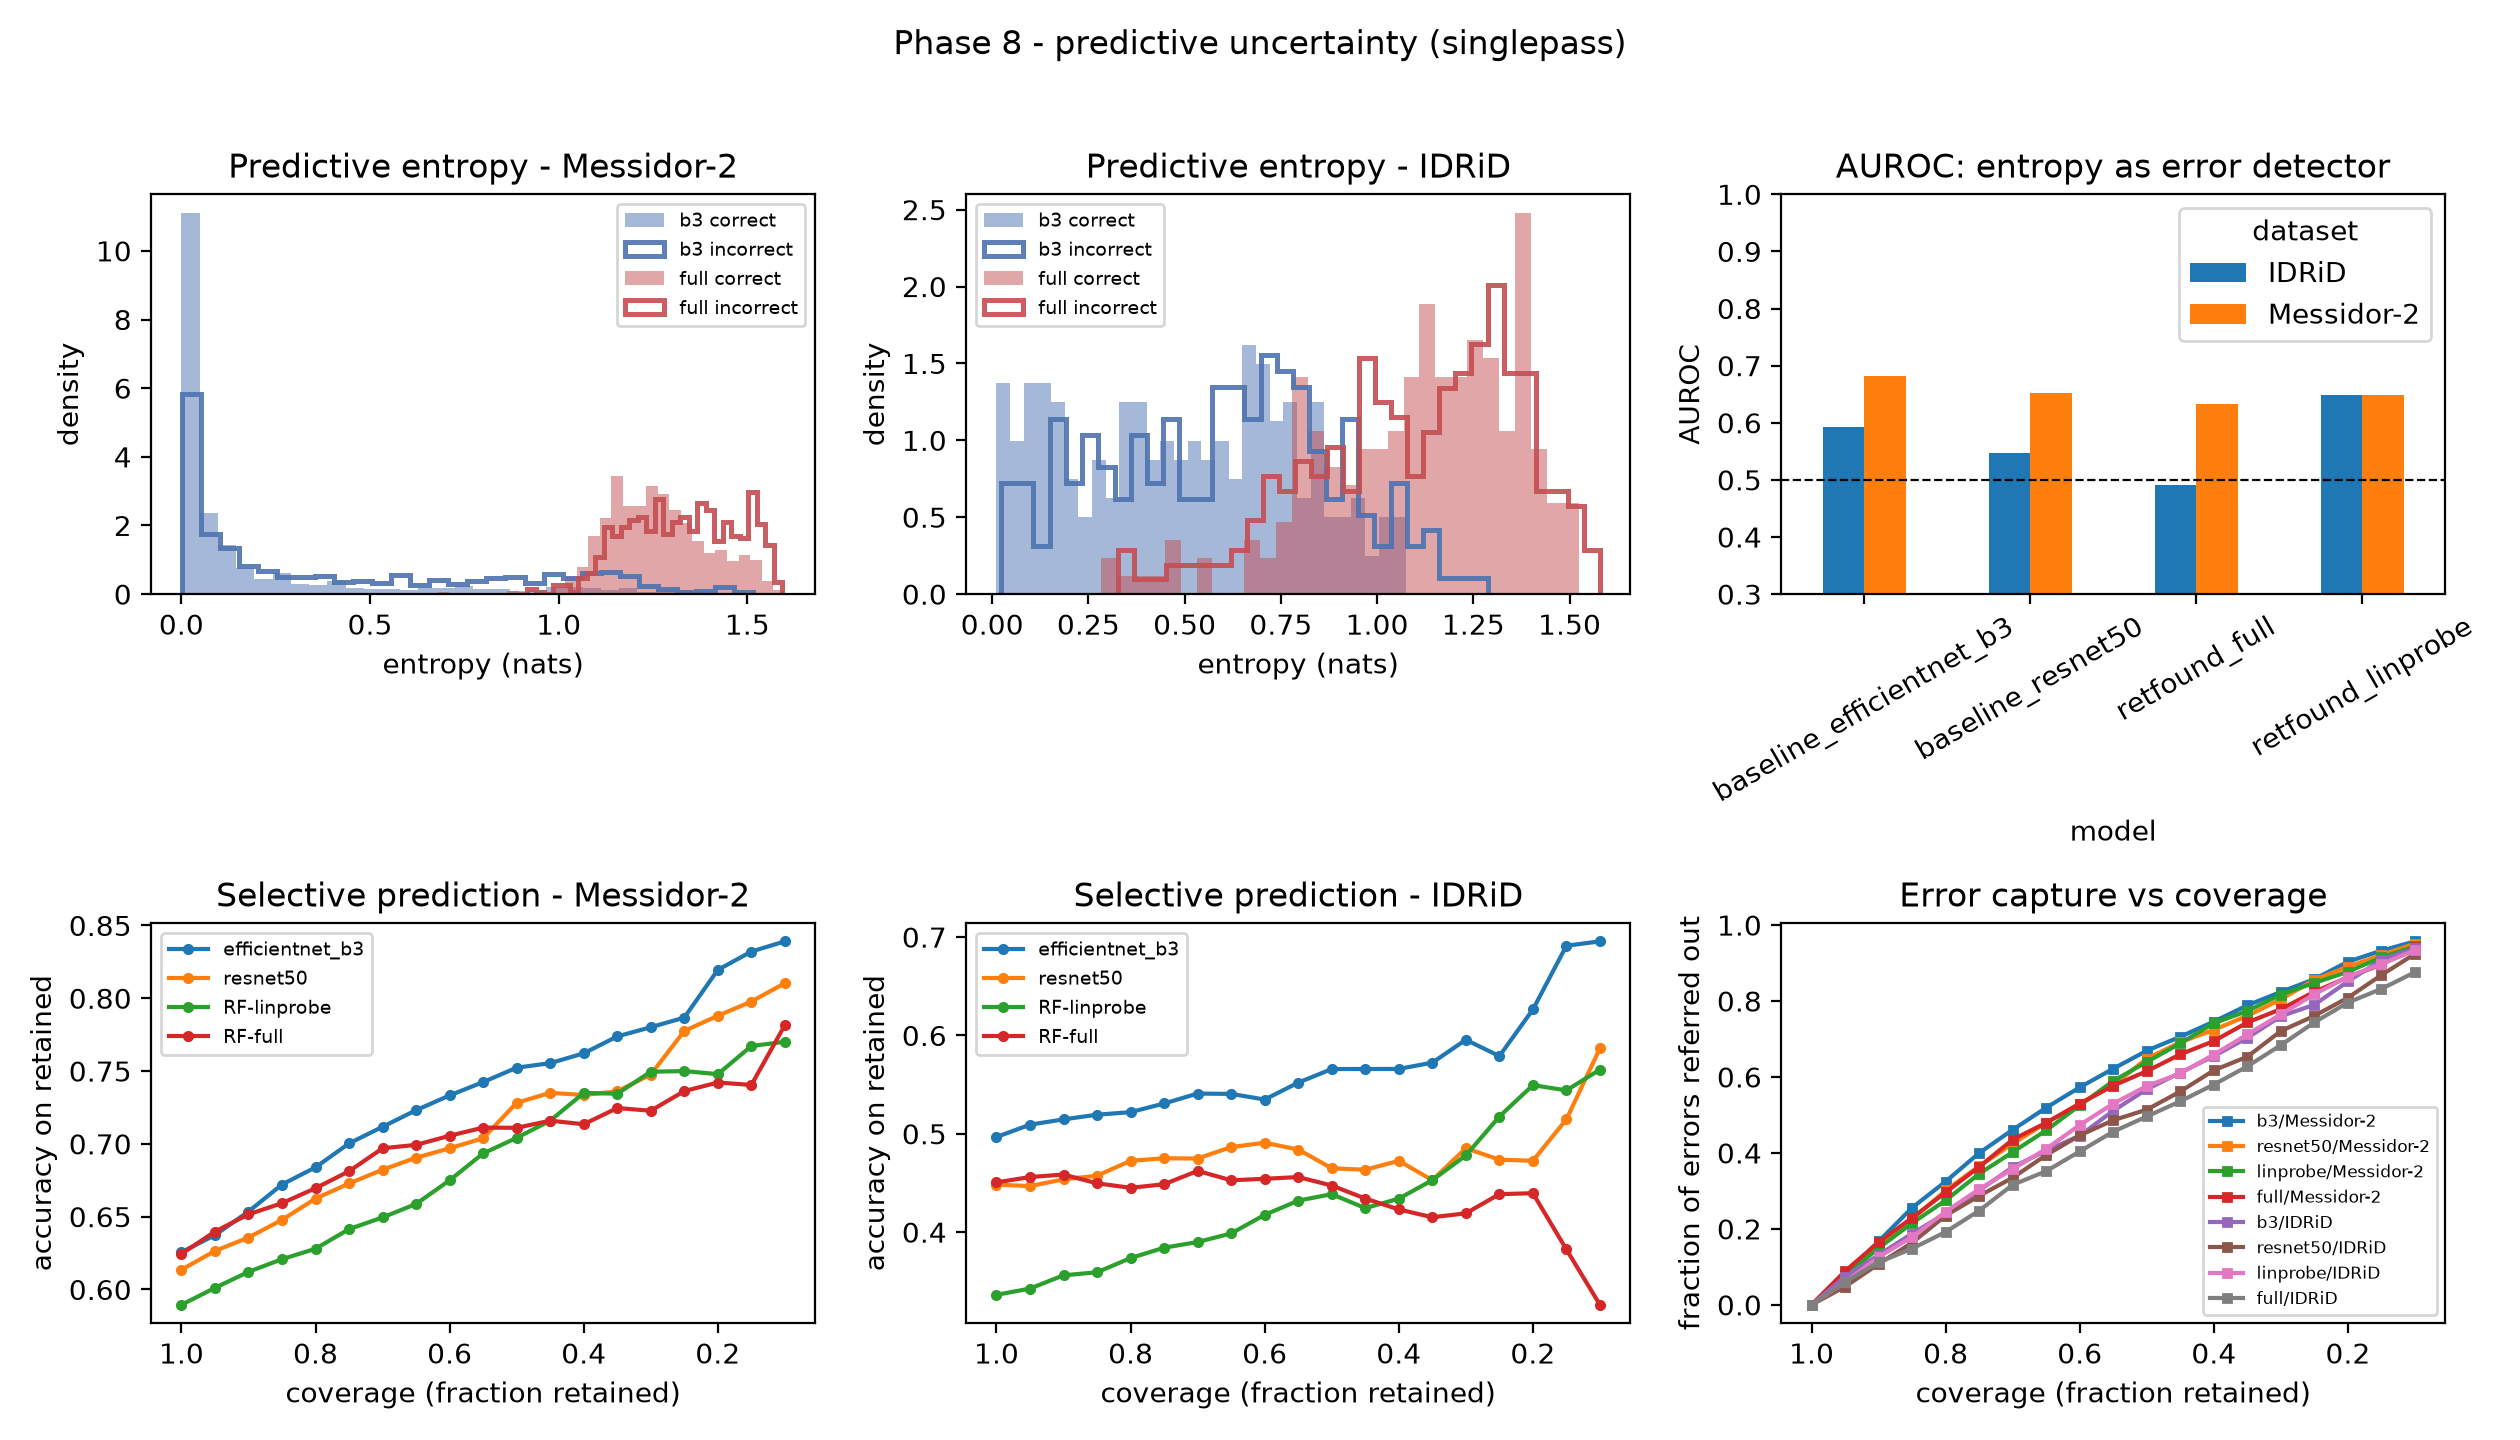
\includegraphics[width=0.98\linewidth]{../outputs/phase8/fig_uncertainty_singlepass.png}
\caption{Predictive uncertainty on external data. Left: predictive-entropy
distributions for correctly and incorrectly classified images. Centre: AUROC of
predictive entropy as an error detector (dashed line, chance). Right:
selective-prediction curves (accuracy on retained cases, and fraction of all
errors referred out, versus coverage) (\texttt{scripts/phase8\_uncertainty.py}).}
\label{fig:unc}
\end{figure}

% ---------------------------------------------------------------------
\section{Discussion}
\label{sec:discussion}

\paragraph{RQ1 -- Performance.} Under a matched preprocessing, fine-tuning, and
evaluation protocol, fine-tuning RETFound on APTOS~2019 did not yield better
cross-dataset generalisation for five-class DR grading than an
ImageNet-pretrained CNN; on the pre-specified contrasts it generalised
\emph{worse}. Both RETFound variants lost significantly more ordinal agreement
than the EfficientNet-B3 baseline on Messidor-2 (difference in QWK drop with a
95\% CI excluding zero), and the baseline had a significantly higher referable-DR
AUC on both external datasets by DeLong's test while being statistically
indistinguishable from all models internally. The direction was consistent
across linear probing -- which ran to a clean early stop -- and full fine-tuning,
so it is not an artefact of the early-stopped full run. This does not contradict
RETFound's reported strengths on other tasks and modalities, but it tempers the
expectation that retinal-domain self-supervised pretraining automatically confers
robustness to the specific shifts represented by Messidor-2 and IDRiD (different
cameras, acquisition, populations, and -- for Messidor-2 -- an adjudicated
reference standard). One plausible reading is that full fine-tuning on a
single moderately sized dataset (APTOS, $\approx$2.6k training images) allows a
large ViT to fit APTOS-specific acquisition characteristics at least as readily
as it exploits its pretrained retinal features.

\paragraph{Nature of the shift.} The Messidor-2 collapse is an ordinal-structure
failure: models predict almost exclusively grade~0 or grade~2, so accuracy is
partly preserved by the high grade-0 prevalence while QWK falls sharply. The
IDRiD pattern is different -- a base-rate shift toward more advanced disease --
so accuracy falls more than QWK. Reporting balanced accuracy alongside QWK
(Table~\ref{tab:master}) separates these effects, and we recommend this practice
for external-validation studies generally.

\paragraph{RQ2 -- Explainability.} Neither model family produced more
clinically plausible saliency overall, but the two behaved differently under the
harder shift. On IDRiD both the CNN Grad-CAM++ and the method-matched
Vision-Transformer Grad-CAM concentrated on retinal tissue away from the optic
disc and border ($\geq$83\% proxy-plausible). On Messidor-2 the CNN saliency
stayed on-tissue even for misclassified images, whereas RETFound's saliency moved
substantially to the image periphery -- and did so most for its errors. This is
consistent with the performance result: under the Messidor-2 shift the foundation
model appears to rely more on image-level acquisition cues than on focal lesions.
Because plausibility here is scored by an automated proxy on 20 images per
cell, the effect should be read as hypothesis-generating and confirmed with
blinded expert grading.

\paragraph{RQ3 -- Uncertainty.} Predictive uncertainty was, at best, a weak
safeguard under dataset shift. Entropy separated correct from incorrect
predictions internally (AUROC up to 0.84) but only weakly externally (0.55--0.68),
and for the RETFound full fine-tune on IDRiD it carried no error signal at all.
In operational terms, referring the most-uncertain 10\% of external predictions
would capture only about 10--18\% of the errors -- barely better than referring a
random 10\%. An uncertainty-gated referral step is therefore not, on this
evidence, a sufficient deployment safeguard for these models on these shifts;
calibration and out-of-distribution detection tailored to the deployment domain
would be needed.

\paragraph{Comparison with the literature.} Reported internal QWK for five-class
DR grading on APTOS is typically 0.88--0.93, matching our internal values
(0.85--0.88). External-validation reports for DR AI more often use referable-DR
sensitivity/specificity than five-class QWK, and internal-to-external QWK drops
of the magnitude seen here (0.38--0.50 on Messidor-2) are seldom reported because
five-class external validation on an adjudicated reference standard is itself
uncommon \citep{grzybowski2020review}. Where cross-population degradation of DR
models has been quantified it is substantial \citep{dai2021spectrum,beede2020},
and our results extend that observation specifically to a retinal foundation
model under a matched protocol. The Messidor-2 adjudicated grades
\citep{krause2018} are a stricter target than the single-grader APTOS labels,
which likely contributes to the size of the drop for every model.

\paragraph{Limitations.}
(i) The RETFound full fine-tuning results use an epoch-6 checkpoint (validation
QWK \num{0.935}). Two attempts to run the planned 30-epoch schedule to completion
on the available hardware were curtailed -- the first by a
checkpoint-synchronisation I/O slowdown, the second by host memory exhaustion
after the model had already converged. In the second attempt the validation QWK
plateaued at $\approx$\num{0.94} from epoch~16 onward (best \num{0.943} at
epoch~19), essentially matching the value at which the first run was stopped, so
the epoch-6 checkpoint is representative of the converged model; its values are
marked \textsuperscript{p} pending a clean completed run in a memory- and
throttle-unconstrained environment. The negative conclusion does not depend on
this: it also holds for the RETFound linear-probe variant, which ran to a clean
early stop, and the full-fine-tune Messidor-2 deficit (difference in QWK drop
\prov{$+0.124$}, 95\% CI \numrange{0.074}{0.175}) is far larger than the
$\leq \num{0.01}$ validation-QWK headroom between epoch~6 and convergence.
(ii) All datasets are retrospective and public; no prospective or
clinical-deployment claim is made.
(iii) The IDRiD Disease-Grading mirror used contained 455 of 516 images; because
it is an external test set this cannot bias model development, and the subset
spans all five grades with the full release's class mix, but precision is
correspondingly reduced.
(iv) External sample sizes limit precision for rare grades -- grade-1 (mild)
sensitivity is effectively not estimable on Messidor-2 for any model -- and some
bootstrap CIs are correspondingly wide.
(v) Explainability plausibility was scored by a transparent automated proxy, not
by a blinded expert grader, and the proxy cannot exclude vessel-centred
activation; 20 images were rated per model per external dataset. A blinded
two-rater assessment with Cohen's~$\kappa$ would strengthen RQ2.
(vi) A single foundation model (RETFound masked-autoencoder, colour-fundus
weights) and a single downstream task (five-class DR grading) were studied; the
result should not be generalised to other retinal foundation models or tasks
without direct testing.
(vii) Model calibration was not formally assessed (reliability diagrams, expected
calibration error); this is left as future work.

\paragraph{Clinical and practical implications.} The magnitude of the
internal-to-external drop -- for every model, foundation or not -- reinforces
that internal test performance is a poor guide to behaviour on new data, and
that external validation and, where possible, an uncertainty-aware referral
mechanism should precede any screening deployment.

% ---------------------------------------------------------------------
\section{Conclusions}

In this retrospective external-validation study, a fine-tuned retinal foundation
model did not outperform a standard ImageNet-pretrained CNN for cross-dataset
diabetic retinopathy grading, and by the pre-specified comparisons -- the
difference in internal-to-external QWK drop and the DeLong referable-DR AUC
comparison -- it performed worse on the harder external dataset. All models
lost substantial ordinal agreement on independent data, most severely on
Messidor-2; predictive uncertainty was a weak safeguard under that shift; and the
foundation model's saliency became peripheral rather than lesion-centred. These
results argue for external validation, on an independent adjudicated reference
standard where possible, as the primary evidence standard for retinal AI, and
show that neither retinal-domain pretraining nor an uncertainty threshold can be
assumed to deliver deployment-ready robustness on its own.

% ---------------------------------------------------------------------
\section*{Declarations}

\subsection*{Data and Code Availability}
\label{sec:availability}
Analysis code, split image-ID lists, per-image prediction files, and the
environment specification are available at \todo{repository URL / DOI}. The three
datasets are third-party and are not redistributed: APTOS~2019 via Kaggle
\citep{aptos2019}; Messidor-2 via ADCIS \citep{decenciere2014} with adjudicated
grades from \citep{krause2018}; IDRiD via IEEE DataPort \citep{porwal2018}. See
\texttt{DATA\_PROVENANCE.md} for URLs, versions, access dates, and licences.

\subsection*{Ethics}
This study analysed only previously published, fully de-identified, publicly
available retinal image datasets (APTOS~2019, Messidor-2, IDRiD), each collected
and graded under the ethical approvals and consent procedures of its original
study. No new human-subjects data were collected and no individual can be
identified from the data used. Institutional review board review was therefore
not required for this secondary analysis.
\todo{Replace the preceding two sentences with the target journal's exact
required wording for secondary use of public, de-identified data, and add an
institutional ethics-waiver statement if your institution requires one.}

\subsection*{Funding}
\todo{State the funding source(s) and grant numbers, or: ``This research received
no external funding.''}

\subsection*{Conflicts of Interest}
\todo{Declare each author's competing interests, or: ``The authors declare no
conflict of interest.''}

\subsection*{Author Contributions}
\todo{Assign CRediT roles per author, e.g. Conceptualization, Methodology,
Software, Formal analysis, Data curation, Writing -- original draft, Writing --
review \& editing, Visualization, Supervision.}

\subsection*{Use of AI tools}
Data preprocessing, model-training, evaluation and statistical code, the
manuscript figures, and portions of the manuscript text were prepared with the
assistance of an AI coding assistant under author supervision; all analyses were
executed by the authors, and all results, interpretations, and the final text
were verified and approved by the authors, who take full responsibility for the
work. \todo{Adjust this disclosure to match the target journal's AI-use policy
and the actual division of labour.}

% ---------------------------------------------------------------------
\bibliographystyle{plainnat}
\bibliography{references}

\end{document}
